\chapter[Workshop Connected Minds]{Workshop zur Bestimmung eines Aktionssets}\label{cha:Workshop}
Um ein Konzept für unser Modell abzuleiten, interessiert uns welche Arten von Interaktionen, in einem Auto stattfinden und aus welchen Einzelschritten diese bestehen. Darüber hinaus wollen wir aktuelle und mögliche Umsetzungen der Modalitäten Haptik, Touch, Sprache und Gestik zu den Einzelschritten sammeln. Die Interaktionen sollen in die Kategorien Kommunikation, Navigation, Medien, Komfortfunktionen und Einstellungen unterteilt werden.

Zu diesem Zweck wollen wir im Rahmen eines Workshops unsere Ziele erarbeiten. Dafür ist eine Fokusgruppe geeignet, die sich im automobilen Bereich befindet.   
Bei BMW gibt es jeden Mittwoch die Möglichkeit eine Brainstorming Runde (Connected Minds) mit freiwilligen internen Mitarbeitern anzumelden. Diese Möglichkeit nutzen wir, um unseren Workshop durchzuführen.
Am 24.08.2016 führten wir mit insgesamt neun Teilnehmern unseren Workshop durch. 
Wir bereiteten unsere Ziele vor, die es zu erreichen galt. Die Ziele lauten wie folgt:  
\begin{enumerate}
	\item \textbf{Ziel:} Anwendungsbeispiele von Interaktionen im Auto sammeln und diese einer der Kategorien zuordnen (Kommunikation, Navigation, Medien, Komfortfunktionen und Einstellungen). Anschließend diese in ihre einzelnen Aktionen zerlegen. 
	\item \textbf{Ziel:} Aus den Anwendungsbeispielen die Aktionen gruppieren und Umsetzungen für die verschiedenen Modalitäten (Haptik, Sprache, Touch und Geste) finden beziehungsweise sammeln.
\end{enumerate}
\section[Ablauf]{Organisation und Ablauf des Workshops}
\begin{figure}[ht]
  \centering
  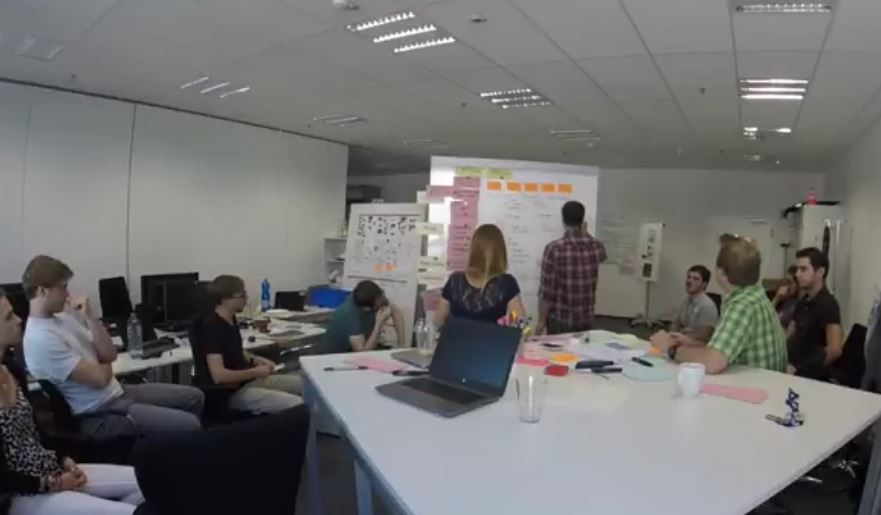
\includegraphics[width=1\textwidth]{img/ConnectedMind.jpg}
  \caption{Connected Minds bei BMW}
  \label{fig:ConnectedMind}
\end{figure} 
Nach einer kurzen Vorstellrunde wurden die Teilnehmer in das Thema eingewiesen und die zwei zu erreichenden Ziele vorgestellt. 
Für das erste Ziel sammelten wir im ersten Schritt Anwendungsbeispiele und ordneten sie den Themengebieten Kommunikation, Navigation, Medien, Komfortfunktionen oder Einstellungen zu (siehe \fref{fig:ConnectedMindErgebnisse} linkes Bild).
\begin{figure}[ht]
  \centering
  \includegraphics[width=1\textwidth]{img/ConnectedMindsErgebnis.jpg}
  \caption[Connected Minds Ergebnisse]{Connected Minds Ergebnisse - Ziel 1 (links), Ziel 2 (rechts)}
  \label{fig:ConnectedMindErgebnisse}
\end{figure}  

Als nächsten Schritt gliederten wir jedes Anwendungsbeispiel in die jeweiligen Aktionen, wobei wir darauf achteten, dass sie möglichst abstrakt und vom Interface unabhängig formuliert wurden. 
Ein Beispiel hierfür ist Abfolge von etwas Auswählen, Inkrementieren und Bestätigen. 
Die gesammelten Aktionen wurden für das zweite Ziel gruppiert und anschließend auf einer neuen Tafel untereinander gepinnt. 
Für jede Aktion wurden sowohl aktuell bestehende als auch potentiel mögliche Umsetzungen für die Modalitäten Haptik, Touch, Geste und Sprache gesammelt (siehe \fref{fig:ConnectedMindErgebnisse} rechtes Bild und \fref{tab:table1}). 

Um die Ziele zu erreichen benötigten wir insgesamt 1,5 Stunden, wobei das erste Ziel nach 30 Minuten erfüllt wurde und das zweite Ziel eine Stunde benötigte. 
Der Workshop wurde auf Video aufgezeichnet.
\section[Ergebnisse des Workshops]{Ergebnisse des Workshops Connected Minds}
Es haben sich sechs verschiedene Aktionen herauskristallisiert, aus denen alle Bedienbeispiele zusammengesetzt werden können.
\begin{itemize}
	\item \textbf{Bestätigung (B):} Eingabe oder Auswahl bestätigen.
	\item \textbf{Direktauswahl (DA):} Auswahl aus sichtbaren Elementen.
	\item \textbf{Ein-/Ausschalten (E/A):} Ein- und Ausschalten oder Aktivieren und Deaktivieren von Funktionen.
	\item \textbf{Listennavigation (L):} Seitenweise inkrementieren und anschließende Direktauswahl (DA).
	\item \textbf{De-/Inkrementieren (Inkr):}  Scrollen, Erhöhen/Verringern von Werten.
	\item \textbf{Texteingabe (T):}  Wiederholte Eingabe eines Buchstabens und anschließende Bestätigung (B).
\end{itemize}

\begin{table}[ht]
	\centering
	\begin{tabular}{|l|l|l|l|l|}
		\hline
		Aktion & Haptik & Touch & Gesten 			& Sprache\\
		\hline
				\multirow {3}{*}{B}
					& Button drücken		& Tap 				& Daumen hoch, 									& Ja,\\
					& Dreh-Drücker			& 						& Tauch OK, 										& OK,\\
					& 									& 						& bestimmte Geste halten 				& passt\\
		\hline
				\multirow{2}{*}{DA}
					& Button drücken		& Swipe  			& 3D-Pointing 								& Objekt/Funktion \\
					& Dreh-Drücker			& Tap					& 														& benennen \\		
		\hline
				\multirow{2}{*}{E/A}
					& Button (on/off)		& Tap,  			& von offener zu 								& Funktionsname\\
					& Kippschalter			& Swipe				& geschlossener Hand						& "`ein"'/"`aus"'\\
		\hline
				\multirow{3}{*}{L}
					& Button drücken		& Swipe				& relative  										& hoch/runter mit\\
					& 									& 						& Handbewegung									& Start/Stop,\\
					& Dreh-Drücker			& Tap 				& (Wischgeste, Swipe), 					& weiter/zurück,\\
					& 									& Scroll			& Drehbewegung des Fingers 			& Tonhöhe variieren\\		
		\hline
				\multirow{3}{*}{Inkr.}		
					& Button drücken		& Swipe				& relative Handbewegung 				& hoch/runter mit\\
					& 									& 						& 															& Start/Stop,\\
					& Dreh-Drücker			& Tap 				& (Wischgeste, Swipe), 					& weiter/zurück,\\
					& Hebel drücken			& Scroll			& Drehbewegung des Fingers			& Tonhöhe variieren\\					
		\hline
				\multirow{3}{*}{T}
					& Tastatur					& X mal Tap 	& In der Luft schreiben, 				& diktieren,\\
					& Dreh-Drücker			& Schreiben		& 3D-Pointing auf Tastatur,			& sprechen\\		
					& Morsecode					& 						& L auf Tastatur								&  \\	
		\hline			
  \end{tabular}
	\caption{Ergebnisse der Umsetzungsmöglichkeiten der Modalitäten für die verschiedenen Aktionen}
	\label{tab:table1}
\end{table}
Für die sechs Aktionen wurden für die Modalitäten Haptik, Touch, Geste und Sprache vorhandene oder mögliche Umsetzungen gesammelt. 
\fref{tab:table1} listet alle Vorschläge der verschiedenen Modalitäten auf.
Wir entschieden uns bei dem Touchmodus immer für den direkten Touch auf einem Display. TODO(den satz laenger und umformulieren) 
In der schon erwähnten Bachelorarbeit von \citet{stracke2014touch} erwiesen sich diese Varianten bei Touch für eine gute Umsetzung mit schnellen Interaktionszeiten. 
Auch \citet{Rumelin:2013} bekamen beim direkten Touch die besten Zeiten für das vollenden einer Aufgabe.

Um den Umfang der geplanten Studie im realistischen Bereich zu lassen, haben wir uns entschieden die Haptik als Modalität nicht miteinzubeziehen. 
Unser Fokus soll bei den Modalitäten Touch, Geste und Sprache liegen, auch weil die Haptik im automobilen Kontext bereits in Studien untersucht wurde, siehe \citep{Pettitt_2007}, \citep{schneegass_2009} und \citep{SchneegaB_2011}. 
Die haptische Bedienung stellt natürlich weiterhin einen wichtigen Bestandteil der Interaktion im Auto dar. Da dieser Bereich für uns wegfällt benötigen wir somit die Aktion Ein- und Ausschalten nicht. 
Im nicht haptischen Kontext unterscheidet sich diese Aktion nicht von einer gewöhnlichen Aktivierung eines Buttons.
\paragraph{Geeignete Anwendungsbeispiele:}
Aus den im Workshop genannten Beispielen suchten wir fünf stellvertretende Beispiele heraus, die sowohl alle Aktionen abdecken, als auch zu einem der fünf Themengebiete Navigation, Medien, Komfortfunktionen, Einstellungen und Kommunikation zuzuordnen sind. 
\begin{itemize}
\item navigieren zu Rom, Dorfweg und Kirchengasse (Navigation): DA (Navigation) + DA (Zieleingabe) + T (Ziel) + B (bestätigen)
\item Song "`Happy"' aus beliebten Songs wählen (Medien): DA (Medien) + DA (beliebte Songs) + L ("`Happy"' suchen) + DA ("`Happy"' auswählen)
\item Temperatur um $3^\circ$ erhöhen (Komfortfunktionen): DA (Temperatur) + Inkr. (+ $3^\circ$)
\item Lautstärke erhöhen (Einstellungen): DA (Einstellungen) + Inkr. (von 50\% auf ca. 80\%)
\item Maria Müller aus Kontakten anrufen (Kommunikation): DA (Telefon) + DA (Kontakte) + L ("`Maria Müller"' suchen) + DA ("`Maria Müller"' auswählen)
\end{itemize}
Bei der Einstellung der Lautstärke haben wir uns bewusst für eine grobe Angabe geeinigt (Lautstärke in einem Intervall zwischen 75\% und 85\% erhöhen), da eine genaue Angabe (zum Beispiel um 3 Einheiten verringern) eine unnatürliche Veränderung wäre \citep{stracke2014touch}. 
Unsere Anwendungsbeispiele stellen übliche Anwendungen dar und sind teils in vereinfachter Weise dargestellt, um eine zu hohe kognitive Belastung zu vermeiden. 
Da die Zeiten von Experten gemessen werden sollen, ist es wichtig Fehler und zu lange Bedenkzeiten zu eliminieren und zu minimieren.

Die Inkrementation eines Wertes stellen wir in unseren Beispielen in zwei verschiedenen Varianten dar. 
Einmal soll die Temperatur um 3 Grad erhöht werden, indem durch dreimaliges inkrementieren schrittweise der Wert verändert wird. 
Im Beispiel die Lautstärke von 50\% auf ca. 80\% zu inkrementieren wählen wir einen Slider als Darstellung. 
Hier muss nicht eine Aktion 30 mal angewendet werden, um von 50 auf 80 zu inkrementieren, sondern eine direkte Inkrementation (für die Modalitäten Touch und Geste) soll den Wert verändern. 
Wir unterscheiden also die schrittweise Inkrementation (Inkr. (s)), die für kleine Wertunterschiede Sinn macht und eine direkte Inkrementation (Inkr. (d)), die bei größeren und gröberen Wertunterschieden sinnvoll ist.

Bei der Texteingabe eines Ziels haben wir zur Unterscheidung von kurzen und langen Wörtern 3 verschiedene Ziele mit unterschiedlicher Länge gewählt (Rom, Dorfweg und Kirchengasse). 
Außerdem wurde darauf geachtet möglichst einfach zu schreibende Wörter zu verwenden, um negative Einflüsse in Bezug zu Rechtschreibkenntnissen zu vermeiden. 
Es soll in erster Linie die Zeit gemessen werden, die es benötigt einen Button in bestimmter Größe zu treffen. 
Die mentale Zeit sollte sich auf die Interaktion und das Interface beziehen und nicht auf die Rechtschreibung. 
\section[Idee des Modells]{Abgeleitete Idee für ein multimodales Modell}
Mit unserem Modell sollen sich multimodale Interaktionszeiten vorhersagen lassen, indem sie sich aus den Aktionen Direktauswahl aus sichtbaren Elementen (DA), Bestätigung (B), Listennavigation (L), schrittweiser Inkrementation (Inkr.(s)), direkter Inkrementation (Inkr.(d)), und der Texteingabe (T) zusammensetzen. 
Je nach Modalität unterscheiden sich die Zeiten einer Aktion. 
Außerdem wollen wir herausfinden, welche Kosten bei einem Wechsel von einer Modalität zu einer anderen entstehen. 
Eine Aktion soll in unserem Fall eine durchschnittliche Dauer darstellen, die ein geübter Nutzer benötigt in einem bestimmten Modus die Aktion fehlerfrei auszuführen. 
Ob ein Nutzer sich dabei Zeit lässt oder einmal mehr oder weniger die Hand vom Interaktionsbereich zurück zum Lenkrad nimmt stellt dabei keinen Fehler dar, sondern soll mit in den durchschnittlichen Zeiten berücksichtigt werden. 

Bei den Keystroke-Level Modellen auf Operatorebene gibt es eine "`richtige"' Lösung mit einer bestimmten Anzahl an Operatoren. 
Das ist der schnellste Weg, den Experten verwenden, um eine bestimmte Aufgabe zu lösen. 
Doch bei Interaktionen im Auto lässt sich viel schwieriger eine Abfolge von Operatoren bilden. 
Je nach Nutzer und Situation im Auto werden zum Beispiel mehrere Bewegungen vom Lenkrad hin zum Interaktionsbereich gemacht als nötig. 
Deshalb erscheint es uns eine gute Annäherung die Gesamtdauer in unserem Modell nicht durch Operatoren, sondern durch Aktionen zusammenzusetzen. 
Die Wechselkosten, die wir ebenfalls in unserem Modell berechnen und berücksichtigen wollen enthalten unter anderem einen mentalen Operator und einen Homing Operator \citep{Card_1980} bzw. einen Reach Far Operator \citep{Green_2002}. 
Wie bei dem KLM soll auch bei unserem Modell von Experten ausgegangen werden. 
Es sollen nur Durchgänge gewertet werden, die keine Fehler vom System oder dem Nutzer mit dem System aufweisen.